%%%%%%%%%%%%%%%%%%%%%%%%%%%%%%%%%%%%%%%%%%%%%%%%%%%%%%%%%%%%%%%%%%%%%%%%%%%
% This is LaTeX file for Homework Assignment 3
% Author: Shuo Yang
%%%%%%%%%%%%%%%%%%%%%%%%%%%%%%%%%%%%%%%%%%%%%%%%%%%%%%%%%%%%%%%%%%%%%%%%%%%

\documentclass[11pt]{article}
\usepackage{amsmath,amssymb,epsfig,graphics,hyperref,amsthm,mathtools}
\DeclarePairedDelimiter\ceil{\lceil}{\rceil}
\DeclarePairedDelimiter\floor{\lfloor}{\rfloor}

\hypersetup{colorlinks=true}

\setlength{\textwidth}{7in}
\setlength{\topmargin}{-0.575in}
\setlength{\textheight}{9.25in}
\setlength{\oddsidemargin}{-.25in}
\setlength{\evensidemargin}{-.25in}

\reversemarginpar
\setlength{\marginparsep}{-15mm}

\newcommand{\rmv}[1]{}
\newcommand{\bemph}[1]{{\bfseries\itshape#1}}
\newcommand{\N}{\mathbb{N}}
\newcommand{\Z}{\mathbb{Z}}
\newcommand{\imply}{\to}
\newcommand{\bic}{\leftrightarrow}

% Some user defined strings for the homework assignment
%
\def\CourseCode{CS566}
\def\AssignmentNo{6}
\def\DateHandedOut{Fall, 2015}
\def\Author{Shuo Yang}
\def\GradeID{50}

\begin{document}

\noindent

\CourseCode \hfill \DateHandedOut

\begin{center}
Homework Assignment \#\AssignmentNo\\
Student: \Author\\
GradeID: \GradeID\\
\end{center}

% A horizontal split line
\hrule\smallskip

\vspace{1.5em}
\underline{\textbf{Problem 1}}

\begin{center}
  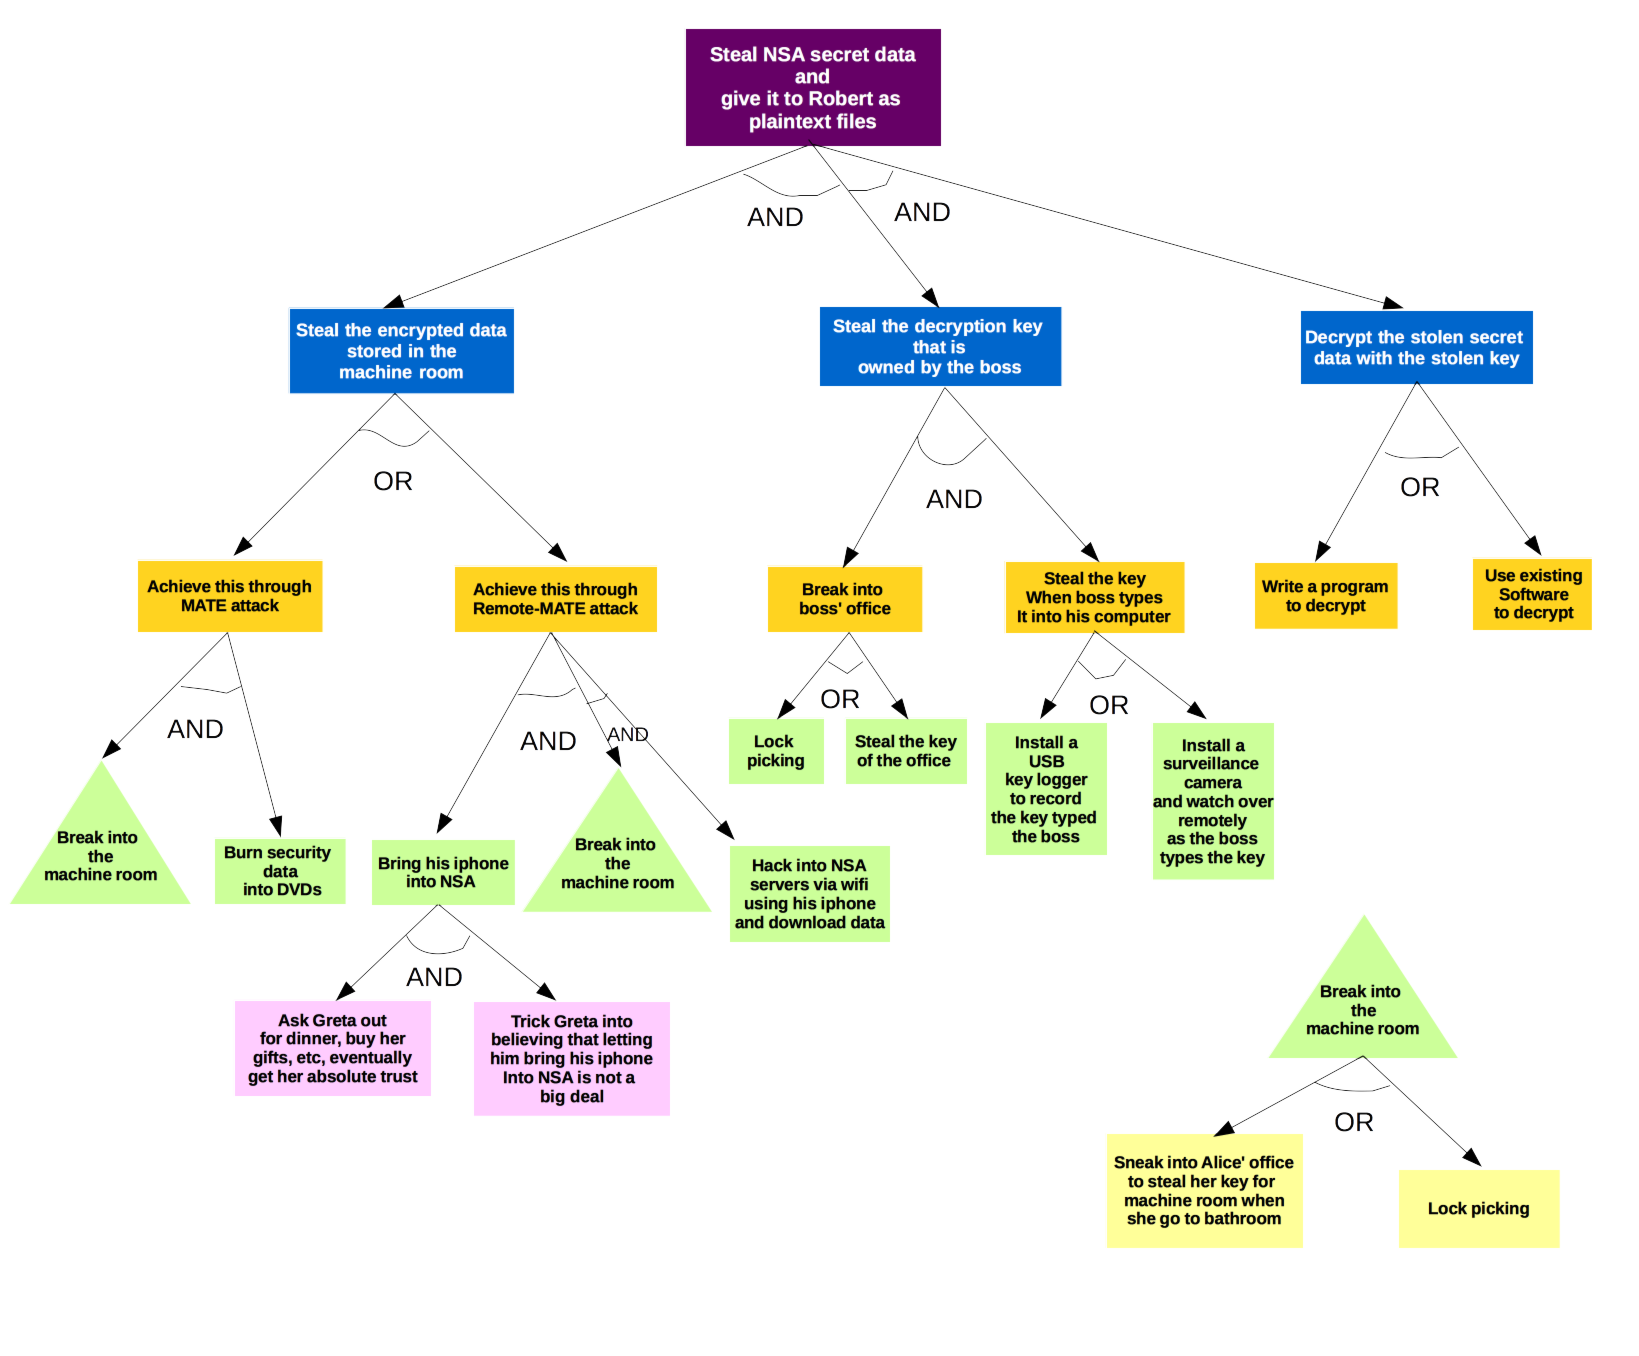
\includegraphics[width=15cm,height=12cm]{./hw6-p1.png}
\end{center}

\underline{\textbf{Problem 2}}
% Enumerate through all questions.
\begin{enumerate}

\item $\phi(210)$

  First, identify the prime factors of 210:\\
  $210 = 2 * 3 * 5 * 7$

  Then, according to Euler's Totient Function:
  
  \begin{align}
    \phi(210) &= 210 * (1-\frac{1}{2}) * (1-\frac{1}{3}) *
    (1-\frac{1}{5}) * (1-\frac{1}{7})\\
    &= 210 * \frac{1}{2} * \frac{2}{3} * \frac{4}{5} * \frac{6}{7}\\
    &= 48
  \end{align}

\item $\phi(187)$

  First, identify the prime factors of 187:\\
  $187 = 11 * 17$

  Then, according to Euler's Totient Function:
  
  \begin{align}
    \phi(187) &= 187 * (1-\frac{1}{11}) * (1-\frac{1}{17})\\
    &= 187 * \frac{10}{11} * \frac{16}{17}\\
    &= 160
  \end{align}

\item $(47^{78}) \mod 79$

  Since $GCD(47, 79) = 1$, 47 is relatively prime to 79. Since 79 is a
  prime number, we know that $\phi(79) = 79 - 1 = 78$.

  Thus according to Euler's Theorem, we have:
  \begin{align}
    (47^{78}) \mod 79 &= (47^{\phi(79)}) \mod 79\\
    &= 1
  \end{align}

\item $(77777777^{2028}) \mod 2029$

  Since 2029 is a prime number (I verified this with a simple Python
  script), $\phi(2029) = 2028$. And since 2029 is not a prime factor
  of 77777777, we know that 77777777 is relatively prime to 2029.

  According Euler's Theorem:
  \begin{align}
    (77777777^{2028}) \mod 2029 &= (77777777^{\phi(2029)} \mod 2029\\
    &= 1
  \end{align}

\item $(223213128736127386218^{7906}) \mod 7907$

  Since 7907 is a prime number (I verified this with a simple Python
  script), $\phi(7907) = 7906$. And since 7907 is not
  a prime factor of 223213128736127386218, we know that
  223213128736127386218 is relatively prime to 7907.

  According Euler's Theorem:
  \begin{align}
    (223213128736127386218^{7906}) \mod 7907 &=
    (223213128736127386218^{\phi(7907)} \mod 7907\\
    &= 1
  \end{align}

\end{enumerate}
\end{document}
